\documentclass{standalone}

\usepackage{rubfonts2009}
\usepackage[scaled=.90]{helvet}
\usepackage{courier}
\usepackage{eulervm}

\usepackage{tikz}
\usetikzlibrary{mindmap,backgrounds}

\usepackage{xcolor}
\definecolor{saphierblau}{cmyk}{1,0.5,0,.6}
\definecolor{RoyalBlue}{cmyk}{1,0.5,0,0}
\definecolor{Black}{cmyk}{0,0,0,0}
\definecolor{alertred}{rgb}{0.80,0.12,0.12}
\definecolor{linkgreen}{RGB}{0,166,0}
\definecolor{ucorange}{cmyk}{0,0.45,0.93,0.04}
\definecolor{lichtgrau}{cmyk}{0.03,0.03,0.03,0.1}

\renewcommand{\familydefault}{\sfdefault}

\begin{document}
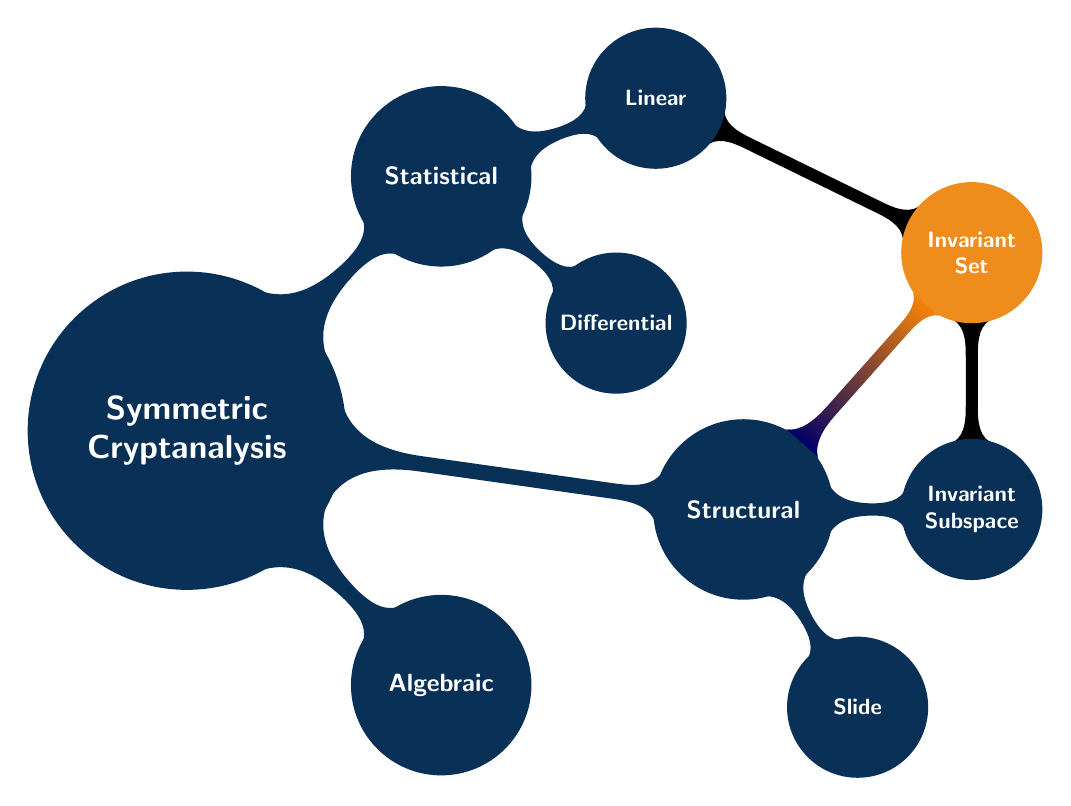
\begin{tikzpicture}[mindmap,
  level 1 concept/.append style={level distance=130,sibling angle=45}]

  \begin{scope}[mindmap, concept color=saphierblau, text=white]
    \node [concept] {\textbf{\large Symmetric Cryptanalysis}}[clockwise from=45]
      child {node [concept] (sta) {\textbf{Statistical}}[clockwise from=20]
        child {node [concept] (lin) {\textbf{Linear}}}
        child {node [concept] (dif) {\textbf{Differential}}}
      }
      child {node [concept] (str) at (2.5, -1) {\textbf{Structural}}[clockwise from=60]
        child [concept color=ucorange] {node [concept] (set) at (1.45, 0.75) {\textbf{Invariant Set}}}
        child {node [concept] (sub) {\textbf{Invariant Subspace}}}
        child {node [concept] (sli) {\textbf{Slide}}}
      }
      child {node [concept] (alg) {\textbf{Algebraic}}};
  \end{scope}

  % Connections of attacks

  \begin{pgfonlayer}{background}
    \path (lin) to[circle connection bar] (set);
    \path (sub) to[circle connection bar] (set);
  \end{pgfonlayer}
\end{tikzpicture}
\end{document}
